tttttt\chapter[Cognitive Radio]{Cognitive Radio}
%\addcontentsline{toc}{chapter}{Chapter 1\\Introduction}
\label{chapter:CR}
In Chapter \ref{chapter:CR}, cognitive radio technology for spectrum sharing is described in detail. Also, as one of the applied technology, spectrum sharing with spectrum database is discussed.

\section{Overview of Cognitive Radio}
Cognitive Radio(CR) is defined as the technology that wireless communication devices are able to be aware of the surrounding environment and configure communication parameters autonomously. Frequency in use, Modulation method, Transmission power all can be treated as communication paramters. Because the adaptive parameter configuration can make an effective usage on White Space possible, it is expected as a solution to the shortage of the spectrum resources.

As a process for Secondary User communication, a series of algorithm named as Cognitive Cycle\cite{ref:mitola} is proposed by J.Mitola I\hspace{-.1em}I\hspace{-.1em}I in 1999. With observing Outside World, Secondary User can obtain various informaiton. Next, after analysis is executed based on information from observation, results are oriented by priority and process is carried out depending on the determined oriented result. If the status has to be responded instantaneously, the appropriate Act needs to be reacted immediately with using the information obtained. For example, when the status of Primary User changes to ON, Secondary User has to stop transmission immediately. Otherwise, in the case that an urgent status exists, an act needs to be determined based on the information. As an example, when Secondary User has an effect on primary signal with huge interfernce power, it is necessary to move to the phase which is stopping transmission or lower the interferece power. If the priority is Normal, an optimised Plan is determined with a long-term observation. While the radio environment changes, the obversation will be observered again. At the end, the Cognitive Cycle is possible based on the process below.
\begin{figure}[!htp]
\begin{center}
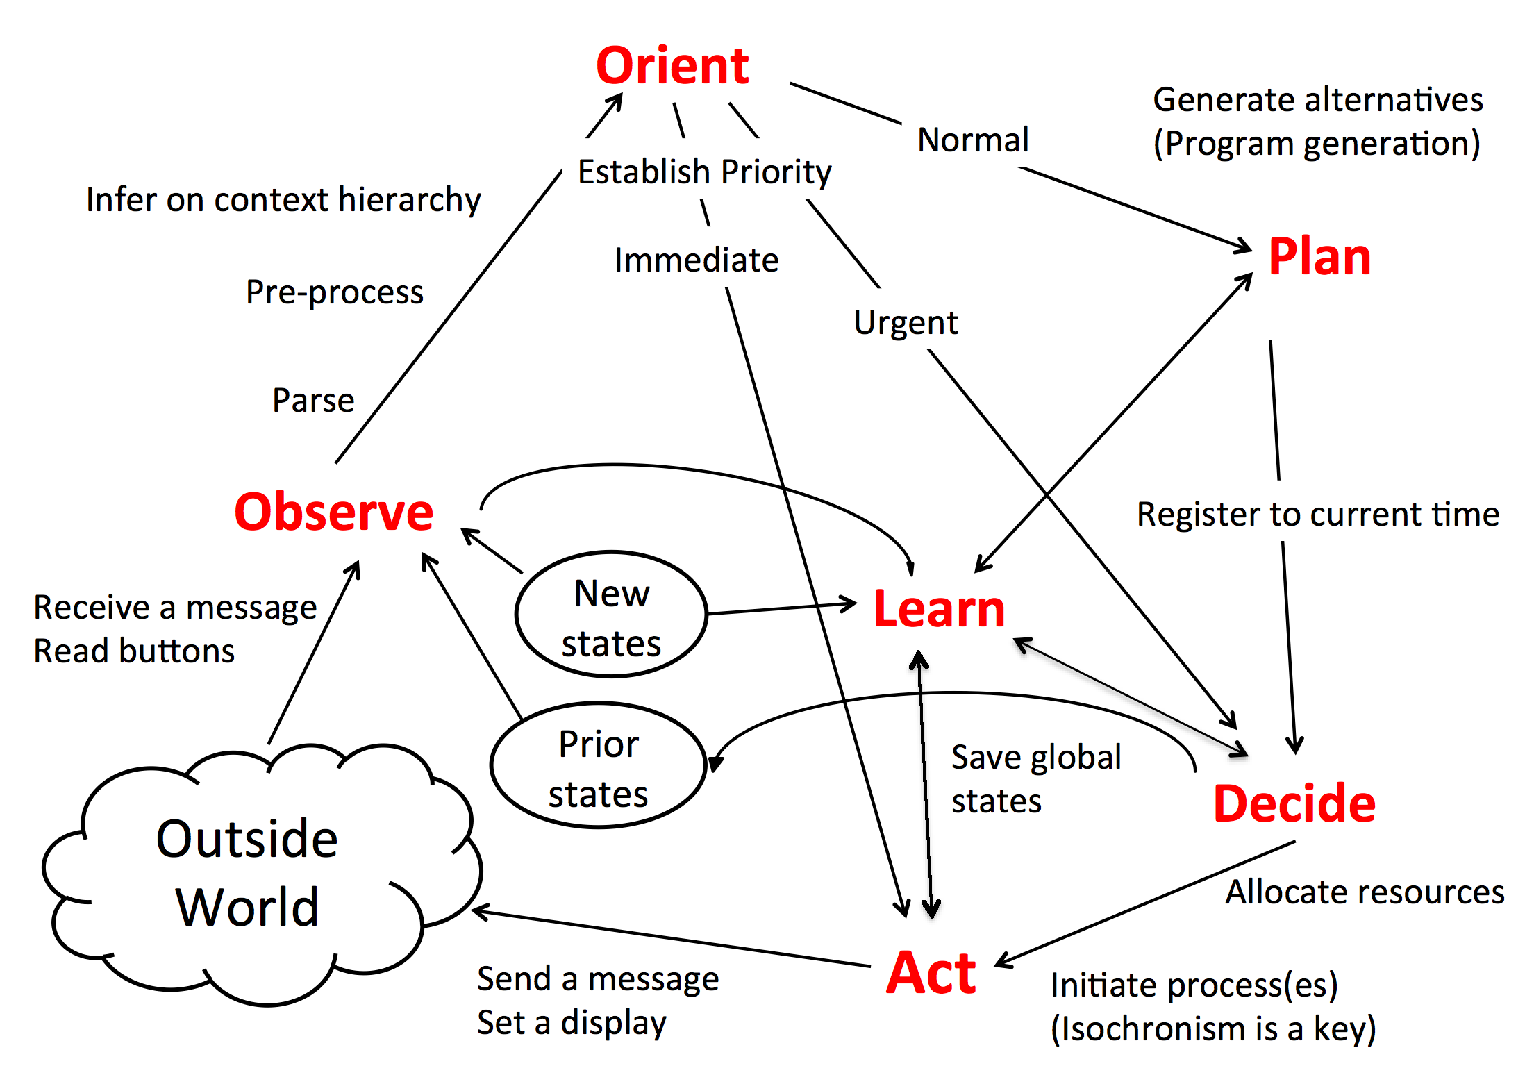
\includegraphics[width=100mm,clip]{cognitive_cycle.eps}
\caption{Cognitive Cycle.}
\label{fig:cognitive cycle}
\end{center}
\end{figure}

The protection of Primary transmission is related to the observation and determination. The signal from Primary User, the own location information from Global Position System(GPS), and the sensing infromation from other nodes can be treated as the observation data. Next, the determination process is optimally executed according to the observation data. Whether the Primary User existence can be determined accurately plays an key role to the cognitive radio sysytems.

In this thesis, we focus on the observe and Orient process in the cognitive cycle for our proposed method.


\section{Dynamic Spectrum Access for Spectrum Sharing}
In the Dynamic Spectrum Access, Secondary Users are able to detect the spectrum and access to it with lower priority than Primary User of that spectrum. The method about how to access to the spectrum is composed of two types, which is defined as Overlay Spectrum Sharing \cite{ref:overlay}and Underlay Spectrum Sharing\cite{ref:underlay}.

\subsection{Overlay Spectrum Sharing}

\begin{figure}[!htp]
\begin{center}
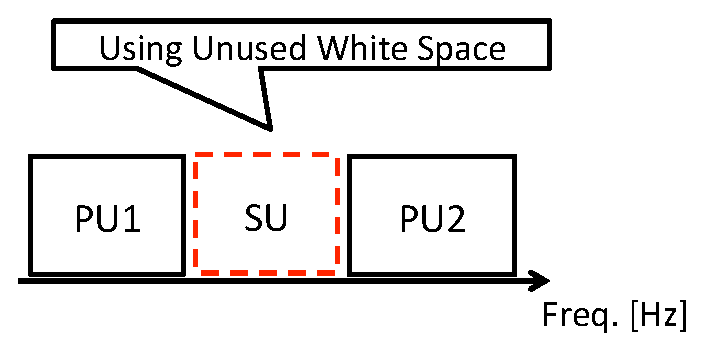
\includegraphics[width=100mm,clip]{overlay.eps}
\caption{Overlay Spectrum Sharing.}
\label{fig:overlay}
\end{center}
\end{figure}

\subsection{Underlay Spectrum Sharing}

\begin{figure}[!htp]
\begin{center}
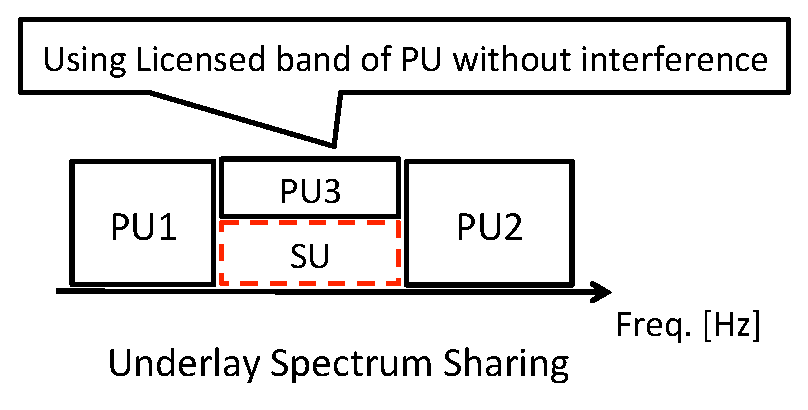
\includegraphics[width=100mm,clip]{underlay.eps}
\caption{Underlay Spectrum Sharing.}
\label{fig:underlay}
\end{center}
\end{figure}

\section{Overview of Spectrum Sharing with Spectrum Database}
